\section{Introduction}

The advent of large language models (LLMs) has established text-to-SQL~\cite{hong2025next,liu2025survey} as a practical interface between users and structured databases.
In real deployments, this interaction is rarely single-turn: users and agents converse over multiple rounds, refining requests and seeking clarification before SQL is produced~\cite{yu2019cosql,huo2026interact}.
Even agents that perform well in single-turn evaluation can fail once conversation becomes part of the task ~\cite{yu2018spider,li2023bird,lei2025spider2}.

\begin{figure}[!t]
    \centering
    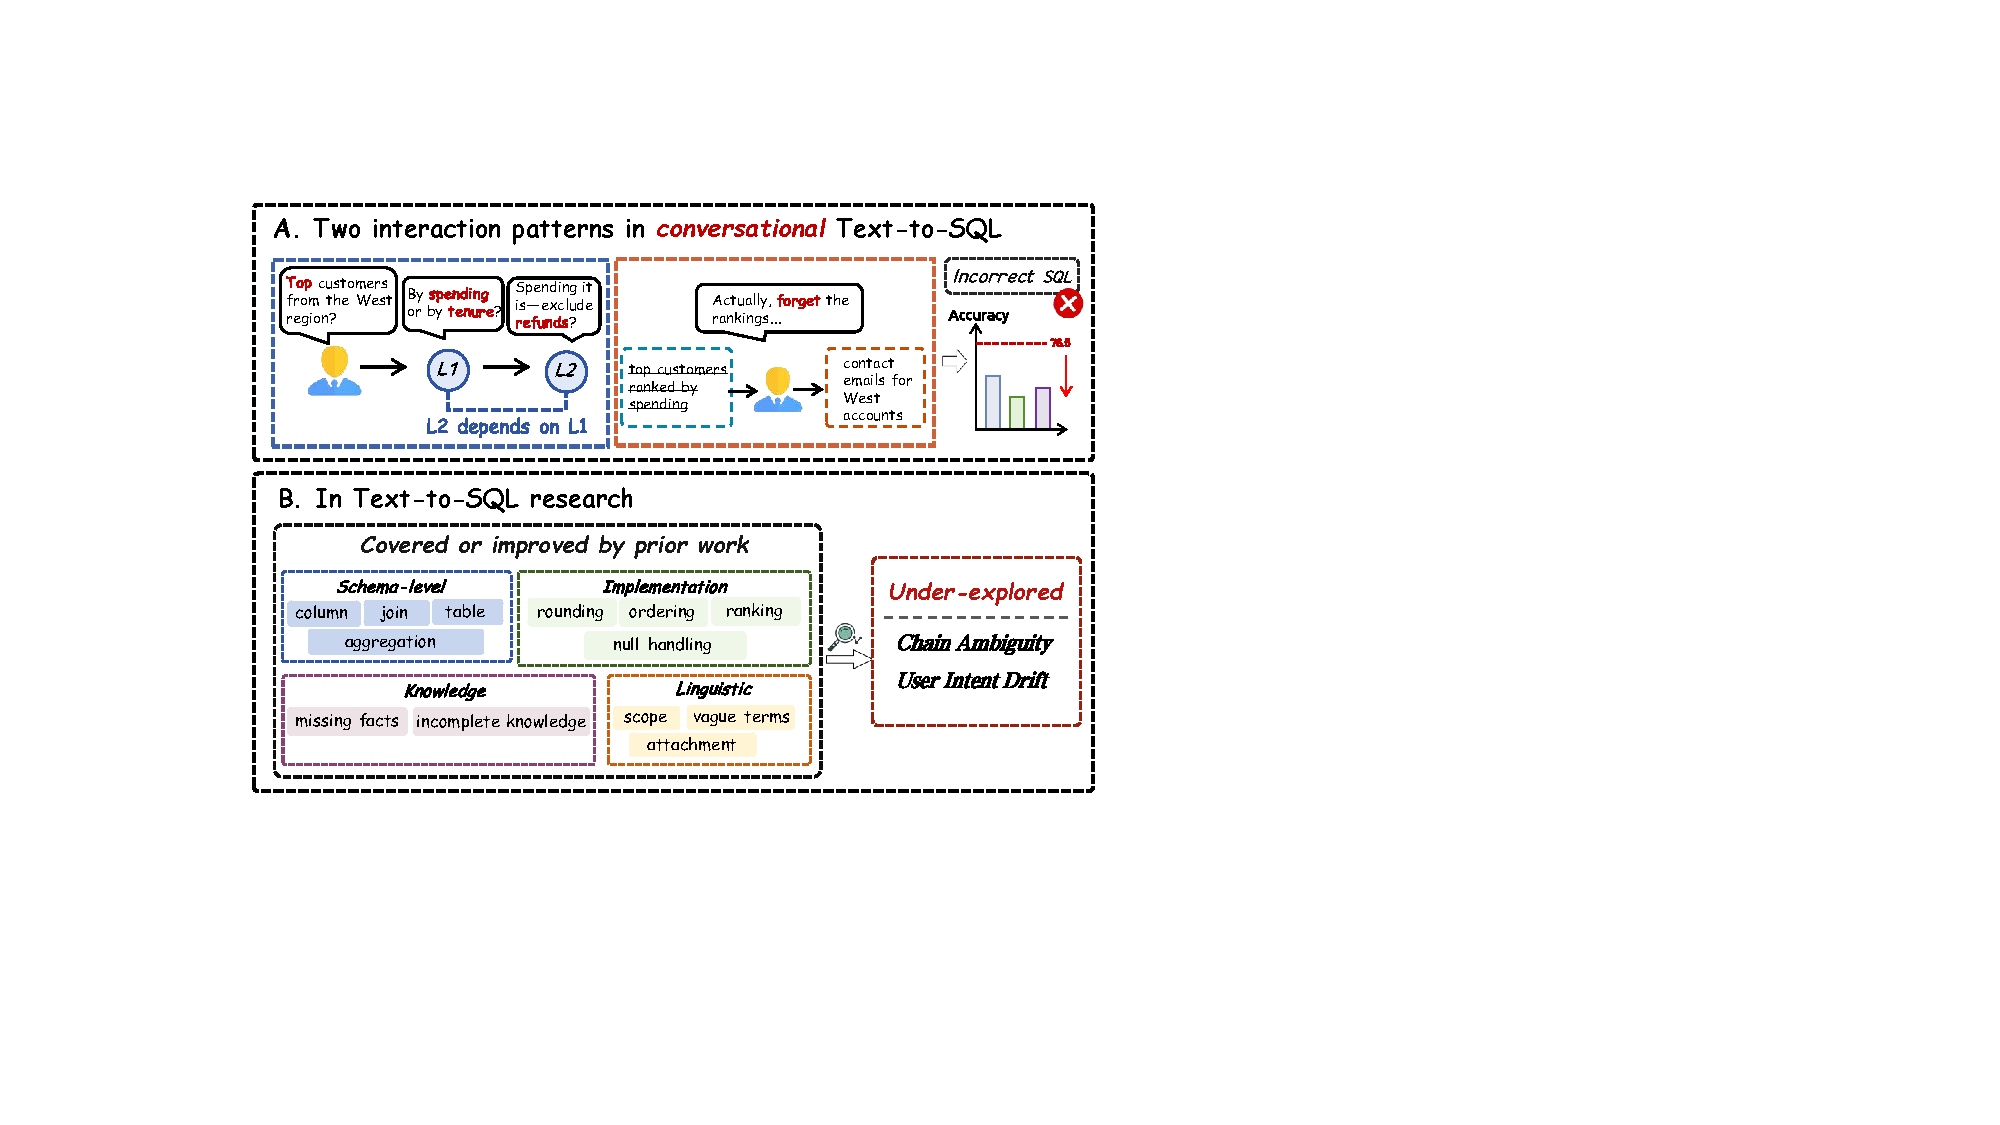
\includegraphics[width=\linewidth]{figure/motivation.pdf}
    \vspace{-6mm}
    \caption{(A) Two conversational patterns that challenge text-to-SQL. (B) Neither is covered by existing text-to-SQL benchmarks or standard evaluation protocols.}
    \label{fig:introduction}
    \vspace{-5mm}
\end{figure}

However, \textbf{how does user intent actually unfold and shift across turns, and are current agents equipped to handle it?}
Figure~\ref{fig:introduction} illustrates two recurring interaction patterns in multi-turn dialogue. First, an underspecified question may trigger \textbf{chain ambiguity}: a layered clarification process in which a later clarification is conditionally dependent on the resolution of an earlier one, going beyond turn-local ambiguity studied in prior work~\cite{bhaskar2023ambiqt,saparina2024ambrosia,dong2025practiq}. Second, a user may retract and replace a committed request element mid-conversation, a non-monotonic shift we term \textbf{user intent drift}. These two interaction patterns raise two critical concerns:
\textbf{1) Chain dependency is not captured by turn-local ambiguity}, as resolving each clarification in isolation says nothing about whether the agent recognizes the dependency between layers;
\textbf{2) Commitment dynamics are not captured by end-to-end accuracy}, as a single execution match cannot tell whether the agent registered the retraction or merely happened to land on the right query.

Existing conversational text-to-SQL benchmarks~\cite{yu2019sparc,yu2019cosql,sun2025dysql,huo2026interact} measure multi-turn SQL accuracy, while a related line of work~\cite{bhaskar2023ambiqt,saparina2024ambrosia,dong2025practiq,ding2026ambisql} also defines turn-local ambiguity taxonomies for individual utterances.
However, these efforts either evaluate dialogue execution as a single end-to-end number or restrict ambiguity to one turn at a time, leaving open how agents handle cross-turn dependency and retraction. In this context, \textbf{effectively evaluating how text-to-SQL agents handle these dialogue-level interaction patterns remains a significant challenge}. As a solution, this paper introduces \textbf{\textsc{TIDE-Bench}}, a benchmark for conversa\textbf{\textsc{ti}}onal text-to-SQL under chain ambiguity and intent \textbf{\textsc{d}}rift \textbf{\textsc{e}}valuation, which operationalizes chain ambiguity through a counterfactual test for conditional dependency and intent drift through a non-monotonicity test over commitment sets derived from SQL abstract syntax trees.

Specifically, \textsc{TIDE-Bench} is built around a paired factorial design over 514 anchor SQLs from BIRD~\cite{li2023bird}: each anchor spawns three samples activating chain ambiguity alone and intent drift alone and together, so that performance differences are attributable to the activated interaction patterns rather than others. The resulting 1,542 samples are produced through a four-stage pipeline with automated validation and human verification. Beyond execution accuracy, \textsc{TIDE-Bench} introduces dedicated metrics for chain-layer identification and drift recognition-resolution. Overall, our main contributions are summarized as follows:
\vspace{-1mm}
\begin{itemize}
\item We identify and formalize \textbf{chain ambiguity} and \textbf{user intent drift} as two underexamined dialogue-level interaction patterns in conversational text-to-SQL, and operationalize each through a counterfactual test for conditional dependency and a non-monotonicity test over commitment sets for systematic evaluation.
\vspace{-2mm}
\item We introduce \textbf{\textsc{TIDE-Bench}}, a benchmark of 514 anchor SQLs and 1,542 paired samples constructed through a four-stage pipeline with automated validation and human verification, whose design attributes performance differences to the activated interaction patterns.
\vspace{-2mm}
\item We evaluate 12 advanced LLMs on \textsc{TIDE-Bench} and also diagnose three key distinct failure modes: a persistent chain identification bottleneck unaffected by ask behavior, a drift recognition-resolution gap concentrated on retraction-target inference, and a joint penalty where the two failures occur on overlapping rather than independent samples.
\end{itemize}